La différence entre les trois algorithmes étudiés réside dans la manière de conjuguer les volumes finis \cite{LeVeque1990} et la multirésolution adaptative.
Le calcul des \textit{flux}, central dans les méthodes volumes finis, 
requiert l'évaluation de termes dépendant de la solution aux \textit{interfaces} amont et avales des cellules.
Les volumes finis n'approximant que les valeurs moyennes sur les cellules et non les valeurs ponctuelles aux interfaces, 
les termes de flux sont alors évalués comme fonction des valeurs moyennes sur les cellules voisines de l'interface.\par
La MRA rend la définition des flux numériques non-univoque - c'est ce qui est ici étudié.\par 
Comme la MRA défini plusieurs grilles de pas $\Delta x,2 \Delta x, 4 \Delta x,...$ il est ambigu de choisir sur quelle grille évaluer les voisins de chaque interface.
En effet, à niveau de détail $l$ fixé, le flux numérique doit-il être déterminé à partir des cellules voisines du niveau $l,l+1,l+2...$ (voir le schéma en fig. \ref{fig:schema_algos}) ? 
Le premier algorithme étudié (la référence en MRA), consiste à évaluer les flux à partir des voisins du même niveau que la cellule étudiée. C'est à dire que 
si flux concerne une cellule de la grille de niveau $l$, les voisines de l'interface sont choisit également au niveau $l$. Cela revient à résoudre localement l'EDP au niveau courant de la grille.
Cet algorithme est la norme en MRA car ne ne requiert aucun calcul supplémentaire, les valeurs sur la grille au niveau $l$ sont directement accessibles.
Le second algorithme consiste à systématiquement les choisir les cellules de la grille la plus fine. Intuitivement c'est le plus précis, mais plus coûteux car 
la grille plus fine n'est pas directement accessible (voir la partie sur la reconstruction en \ref{par:explication_MRA}). 
Enfin le troisième algorithme est un compromis entre les deux approches précédentes. Il consiste à calculer les flux à partir des valeurs un niveau en deçà du niveau courant, 
pour gagner un peu en précision sans pour autant s'exposer à des coûts computationnels prohibitifs.
En \cite{belloti_et_al_2025}, la différence théorique entre les deux premiers algorithmes a été étudiée sur des problèmes d'advection linéaires et
une comparaison expérimentale entre les trois algorithmes a été réalisée sur des problèmes d'advections linéaires et non-linéaires.
\begin{figure}[htpb]
\begin{center}
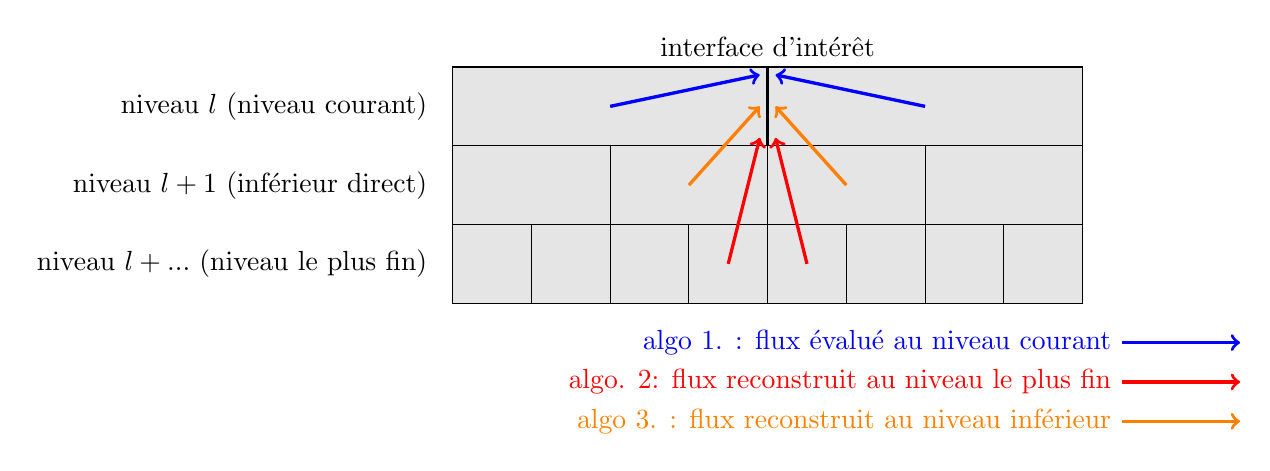
\begin{tikzpicture}
\foreach \i in {0,...,1}{
    \draw[fill=black!10] ({4*\i},0) rectangle ({4*(\i+1)},1);
}
\foreach \i in {0,...,3}{
    \draw[fill=black!10] ({2*\i},-1) rectangle ({2*(\i+1)},0);
}

\foreach \i in {0,...,7}{
    \draw[fill=black!10] ({\i},-2) rectangle ({(\i+1)},-1);
}

\draw[blue, very thick, <-] (3.9,.9) -- (2,.5);
\draw[blue, very thick, <-] (4.1,.9) -- (6,.5);

\draw[orange, very thick, <-] (3.9,.5) -- (3,-.5);
\draw[orange, very thick, <-] (4.1,.5) -- (5,-.5);

\draw[red, very thick, <-] (3.9,.1) -- (3.5,-1.5);
\draw[red, very thick, <-] (4.1,.1) -- (4.5,-1.5);

\draw[black, very thick] (4,0) -- (4,1) node[pos=1, above] {interface d'intérêt};
\node[left] at (-.2,.5) {niveau $l$ (niveau courant)};
\node[left] at (-.2,-.5) {niveau $l+1$ (inférieur direct)};
\node[left] at (-.2,-1.5) {niveau $l+...$ (niveau le plus fin)};

\draw[blue, very thick,->] (8.5,-2.5) -- (10,-2.5) node[pos=0,  left] {algo 1. : flux évalué au niveau courant};
\draw[red, very thick,->] (8.5,-3) -- (10,-3) node[pos=0,  left] {algo. 2: flux reconstruit au niveau le plus fin};
\draw[orange, very thick,->] (8.5,-3.5) -- (10,-3.5) node[pos=0,  left] {algo 3. : flux reconstruit au niveau inférieur};


\end{tikzpicture}
\caption{Illustration des trois algorithmes évalués. L'algorithme 1 en bleu calcul le flux à partir des cellule de la grille au même niveau que l'interface étudiée. 
L'algorithme 2 reconstruit les valeurs de la solution sur la grille de niveau inférieur. L'algorithme 3 reconstruit au niveau le plus fin possible. 
Plus l'algorithme reconstruit finement, plus les valeurs moyennes sont données sur des cellules petites et plus cela s'approche d'une valeur "ponctuelle".}
\label{fig:schema_algos}
\end{center}
\end{figure}